% !TEX options=--shell-escape

\documentclass{report}
\usepackage[T1]{fontenc}
\usepackage{lmodern}

\usepackage{titlesec}
\usepackage{hyperref}

\usepackage[a4paper, margin=2.5cm, headsep=0pt]{geometry}

\usepackage{tgadventor}
\renewcommand{\familydefault}{\sfdefault}

\usepackage{graphicx}
\usepackage{titlepic}
\usepackage[skip=5pt]{caption}

\usepackage[ddmmyyyy]{datetime}
\usepackage[section]{placeins}
\usepackage{enumitem}

\usepackage{minted}
\usepackage[dvipsnames]{xcolor}

\definecolor{bg}{gray}{0.1}

\titleformat{\chapter}{\normalfont\huge}{\bf\thechapter.}{20pt}{\huge\bf}
\titlespacing{\chapter}{0pt}{12pt plus 4pt minus 2pt}{8pt plus 2pt minus 2pt}

\hypersetup{
  colorlinks,
  citecolor=black,
  filecolor=black,
  linkcolor=black,
  urlcolor=blue
}

\graphicspath{technisch verslag imgs/}

\usemintedstyle{monokai}

\newdate{creation}{02}{02}{2022}

\begin{document}
\begin{titlepage}
\centering
\vfill
\bfseries\Huge{Pacenstein\\\large{- Technisch Verslag -}}\\
\normalfont\normalsize\displaydate{creation}
\vfill


\includegraphics[width=\textwidth]{../res/pacenstein.png}
\vfill
\large{
  Lennard Duinkerken\\
  Emma Raijmakers\\
  Daan Roth\\
  Jarno Bröcker
}
\vfill
\end{titlepage}

\tableofcontents

\chapter{Inleiding} % (fold)
\label{cha:inleiding}

% chapter inleiding (end)

\chapter{Game Engine} % (fold)
\label{cha:game_engine}

  \section{Raycasting} % (fold)
  \label{sec:raycasting}
  \subsection{Waarom Raycasting} % (fold)
  \label{sub:waarom_raycasting}
  Dit project gebruikt raycasting om een 2d wereld, op het scherm er uit te laten zien als een 3d wereld. Raycasting is hiervoor gebruikt omdat het een relatief simpele methode is om de wereld 3d te maken. Dit project gebruikt geen hardware acceleratie, dus het is belangrijk dat het een lichte simpele methode is. Vandaar de keuze voor raycasting.
  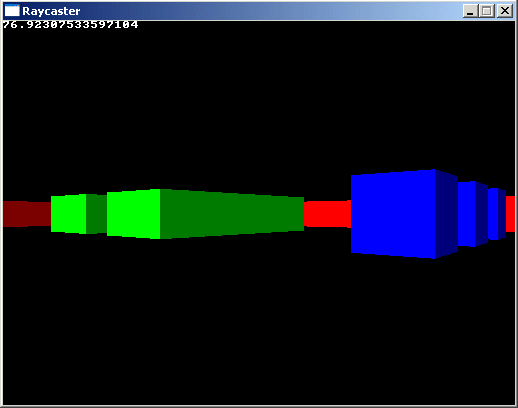
\includegraphics{technisch verslag imgs/raycasteruntextured.png}
  % subsection waarom_raycasting (end)
  % section raycasting (end)

  \section{Game Logic} % (fold)
  \label{sec:game_logic}

  % section game_logic (end)

  \section{Asset Manager} % (fold)
  \label{sec:asset_manager}

  % section asset_manager (end)

  \section{Input Manager} % (fold)
  \label{sec:input_manager}

  % section input_manager (end)

  \section{State Machine} % (fold)
  \label{sec:state_machine}

  % section state_machine (end)
% chapter game_engine (end)

\chapter{States} % (fold)
\label{cha:states}

  \section{Splash} % (fold)
  \label{sec:splash}

  % section splash (end)

  \section{Menu's} % (fold)
  \label{sec:menu_s}

    \subsection{Main Menu} % (fold)
    \label{sub:main_menu}

    % subsection main_menu (end)

    \subsection{Settings Menu} % (fold)
    \label{sub:settings_menu}

    % subsection settings_menu (end)

    \subsection{Leaderboard Menu} % (fold)
    \label{sub:leaderboard_menu}

    % subsection leaderboard_menu (end)

    \subsection{Credits Menu} % (fold)
    \label{sub:credits_menu}

    % subsection credits_menu (end)
  % section menu_s (end)

  \section{In Game} % (fold)
  \label{sec:in_game}

  % section in_game (end)

  \section{Hunting} % (fold)
  \label{sec:hunting}

  % section hunting (end)

  \section{Pause State} % (fold)
  \label{sec:pause_state}

  % section pause_state (end)

  \section{Game Over} % (fold)
  \label{sec:game_over}

  % section game_over (end)
% chapter states (end)

\chapter{Entities} % (fold)
\label{cha:entities}

  \section{Items} % (fold)
  \label{sec:items}

    \subsection{Fruits} % (fold)
    \label{sub:fruits}

      \subsubsection{Apple} % (fold)
      \label{ssub:apple}

      % subsubsection apple (end)

      \subsubsection{Cherry} % (fold)
      \label{ssub:cherry}

      % subsubsection cherry (end)

      \subsubsection{Grape} % (fold)
      \label{ssub:grape}

      % subsubsection grape (end)

      \subsubsection{Peach} % (fold)
      \label{ssub:peach}

      % subsubsection peach (end)

      \subsubsection{Strawberry} % (fold)
      \label{ssub:strawberry}

      % subsubsection strawberry (end)
    % subsection fruits (end)

    \subsection{Ghosts} % (fold)
    \label{sub:ghosts}

      \subsubsection{Blinky - Rood} % (fold)
      \label{ssub:blinky}

      % subsubsection blinky (end)

      \subsubsection{Inky - Cyaan} % (fold)
      \label{ssub:inky}

      % subsubsection inky (end)

      \subsubsection{Pinky - Roze} % (fold)
      \label{ssub:pinky}

      % subsubsection pinky (end)

      \subsubsection{Clyde - Oranje} % (fold)
      \label{ssub:clyde}

      % subsubsection clyde (end)
    % subsection ghosts (end)
  % section items (end)

  \section{Player} % (fold)
  \label{sec:player}

  % section player (end)
% chapter entities (end)

\chapter{Resources} % (fold)
\label{cha:resources}

  \section{UI Elementen} % (fold)
  \label{sec:ui_elementen}

  % section ui_elementen (end)

  \section{Textures} % (fold)
  \label{sec:textures}

  % section textures (end)

  \section{Sprites} % (fold)
  \label{sec:sprites}

  % section sprites (end)

  \section{Afbeeldingen} % (fold)
  \label{sec:afbeeldingen}

  % section afbeeldingen (end)

  \section{Overige} % (fold)
  \label{sec:overige}

  % section overige (end)
% chapter resources (end)

\chapter{Toekomstplannen} % (fold)
\label{cha:toekomstplannen}

% chapter toekomstplannen (end)
\end{document}
